\documentclass[11pt]{article}

% Preamble

\usepackage[margin=1in]{geometry}
\usepackage{amsfonts, amsmath, amssymb}
\usepackage{fancyhdr, float, graphicx}
\usepackage[utf8]{inputenc} % Required for inputting international characters
\usepackage[T1]{fontenc} % Output font encoding for international characters
\usepackage{fouriernc} % Use the New Century Schoolbook font
\usepackage[nottoc, notlot, notlof]{tocbibind}
\usepackage{listings}
\usepackage{xcolor}
\usepackage{karnaugh-map}
% \usepackage[table,xcdraw]{xcolor}

\definecolor{codegreen}{rgb}{0,0.6,0}
\definecolor{codegray}{rgb}{0.5,0.5,0.5}
\definecolor{codepurple}{rgb}{0.58,0,0.82}
\definecolor{backcolour}{rgb}{0.95,0.95,0.92}

\lstdefinestyle{mystyle}{
    backgroundcolor=\color{backcolour},   
    commentstyle=\color{codegreen},
    keywordstyle=\color{magenta},
    numberstyle=\tiny\color{codegray},
    stringstyle=\color{codepurple},
    basicstyle=\ttfamily\footnotesize,
    breakatwhitespace=false,         
    breaklines=true,                 
    captionpos=b,                    
    keepspaces=true,                 
    numbers=left,                    
    numbersep=5pt,                  
    showspaces=false,                
    showstringspaces=false,
    showtabs=false,                  
    tabsize=2
}

\lstset{style=mystyle}

% Header and Footer
\pagestyle{fancy}
\fancyhead{}
\fancyfoot{}
\fancyhead[L]{\textit{\Large{DECA Assignment 3}}}
%\fancyhead[R]{\textit{something}}
\fancyfoot[C]{\thepage}
\renewcommand{\footrulewidth}{1pt}



% Other Doc Editing
% \parindent 0ex
%\renewcommand{\baselinestretch}{1.5}

\begin{document}

\begin{titlepage}
	\centering

	%---------------------------NAMES-------------------------------

	\huge\textsc{
		MIT World Peace University
	}\\

	\vspace{0.75\baselineskip} % space after Uni Name

	\LARGE{
		Digital Electronics and Computer Architecture\\
		Second Year B. Tech, Semester 3
	}

	\vfill % space after Sub Name

	%--------------------------TITLE-------------------------------

	\rule{\textwidth}{1.6pt}\vspace*{-\baselineskip}\vspace*{2pt}
	\rule{\textwidth}{0.6pt}
	\vspace{0.75\baselineskip} % Whitespace above the title



	\huge{\textsc{
			Design and Implementation of Asynchronous counters using\\ JK- Flip flop.
		}} \\



	\vspace{0.5\baselineskip} % Whitespace below the title
	\rule{\textwidth}{0.6pt}\vspace*{-\baselineskip}\vspace*{2.8pt}
	\rule{\textwidth}{1.6pt}

	\vspace{1\baselineskip} % Whitespace after the title block

	%--------------------------SUBTITLE --------------------------	

	\LARGE\textsc{
		Practical Report
	} % Subtitle or further description
	\vfill

	%--------------------------AUTHOR-------------------------------

	\vspace{0.5\baselineskip} % Whitespace before the editors

	\Large{
		Krishnaraj Thadesar \\
		Cyber Security and Forensics\\
		Batch A2, PA 34
	}


	\vspace{0.5\baselineskip} % Whitespace below the editor list
	\today

\end{titlepage}


\tableofcontents
\thispagestyle{empty}
\clearpage


\setcounter{page}{1}
\section{Objectives}
\begin{enumerate}
	\item To understand the operation of Asynchronous counter
	\item To design and implement MOD-N asynchronous counter using JK - Flip flop
\end{enumerate}

\section{Problem Statement}
Design and Implement asynchronous counter using JK- Flip flop

\section{ICs Used}

\begin{enumerate}
	\item IC7400 (NAND Gate)
	\item IC7476 (Dual Master Slave JK Flip Flop)
\end{enumerate}

\section{Platform Used}
Digital Trainer Kit

\section{Theory}

\subsection{Counters}
\textit{A Counter is a device which stores the number of times a particular event or process has occurred, often in relationship to a clock signal}. \\

\noindent
Counters are used in digital electronics for counting purpose, they can count specific event happening in the circuit.

For example, in UP counter a counter increases count for every rising edge of clock. Not only counting, a counter can follow the certain sequence based on our design like any random sequence 0,1,3,2 ...

They can also  be designed with the help of flip flops. The main properties of a counter are timing, sequencing, and counting. Counter  works in two modes
\begin{enumerate}
	\item Up Counter
	\item Down Counter
\end{enumerate}
\subsection{Types of Counters}
Counters are broadly divided into two categories:
\begin{enumerate}
	\item Asynchronous counter
	\item Synchronous counter
\end{enumerate}


\subsection{Asynchronous Counters}
In asynchronous counter we don't use universal clock, only first flip flop is driven by main clock and the clock input of rest of the following flip flop is driven by output of previous flip flops.

The Asynchronous counter is also known as the ripple counter. Below is a diagram of the 2-bit Asynchronous counter in which we used two T flip-flops. Apart from the T flip flop, we can also use the JK flip flop by setting both of the inputs to 1 permanently. The external clock pass to the clock input of the first flip flop, i.e., FF-A and its output, i.e., is passed to clock input of the next flip flop, i.e., FF-B.

\begin{figure}[H]
	\centering
	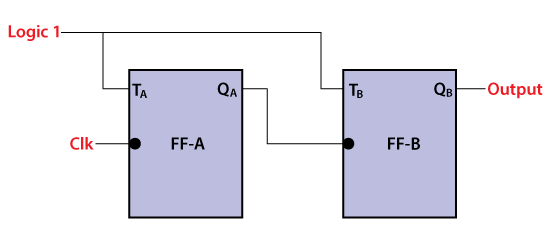
\includegraphics[scale=0.5]{counters2.png}
	\caption{Asynchronous Counter}
\end{figure}
\subsection{Advantages of Asynchronous Counters}
\begin{enumerate}
	\item Asynchronous counters can be easily designed by T flip flop or D flip flop.
	\item These are also called as Ripple counters, and are used in low speed circuits.
	\item They are used as Divide by- n counters, which divide the input by n, where n is an integer.
	\item Asynchronous counters are also used as Truncated counters. These can be used to design any mod number counters, i.e. even Mod (ex: mod 4) or odd Mod (ex: mod3).
\end{enumerate}
\subsection{Applications of Asynchronous Counters}
\begin{enumerate}
	\item They are used as frequency dividers where the frequency of given pulse waveform is divided. Counters are sequential circuit that count the number of pulses can be either in binary code or BCD form.
	\item Asynchronous counters are used as frequency dividers, as divide by N counters.
	\item These are used for low power applications and low noise emission.
	\item These are used in designing asynchronous decade counter.
	\item Also used in Ring counter and Johnson counter.
	\item Asynchronous counters are used in Mod N ripple counters. EX: Mod 3, Mod 4, Mod 8, Mod 14, Mod 10 etc.
\end{enumerate}
\subsection{Involved Truth Tables}

\subsubsection{NAND Gate}

\begin{table}[H]
	\begin{tabular}{|c|c|c|}
		\hline
		{\color[HTML]{000000} \textbf{A}} & {\color[HTML]{000000} \textbf{B}} & {\color[HTML]{000000} \textbf{Q}} \\ \hline
		{\color[HTML]{330001} \textit{0}} & {\color[HTML]{330001} \textit{0}} & {\color[HTML]{F56B00} \textit{1}} \\ \hline
		{\color[HTML]{330001} \textit{0}} & {\color[HTML]{330001} \textit{1}} & {\color[HTML]{F56B00} \textit{1}} \\ \hline
		{\color[HTML]{330001} \textit{1}} & {\color[HTML]{330001} \textit{0}} & {\color[HTML]{F56B00} \textit{1}} \\ \hline
		{\color[HTML]{330001} \textit{1}} & {\color[HTML]{330001} \textit{1}} & {\color[HTML]{F56B00} \textit{0}} \\ \hline
	\end{tabular}
\end{table}
\subsubsection{Truth Table of 3 Bit Asynchronous UP Counter}

\begin{table}[H]
	\begin{tabular}{|c|c|c|c|}
		\hline
		\textbf{\begin{tabular}[c]{@{}c@{}}No of negative or Positive \\ edge of Clock\end{tabular}} & \textbf{\begin{tabular}[c]{@{}c@{}}Q0 \\ LSB\end{tabular}} & \textbf{Q1} & \textbf{\begin{tabular}[c]{@{}c@{}}Q2 \\ MSB\end{tabular}} \\ \hline
		0                                                                                            & 0                                                          & 0           & 0                                                          \\ \hline
		1                                                                                            & 1                                                          & 0           & 0                                                          \\ \hline
		2                                                                                            & 0                                                          & 1           & 0                                                          \\ \hline
		3                                                                                            & 1                                                          & 1           & 0                                                          \\ \hline
		4                                                                                            & 0                                                          & 0           & 1                                                          \\ \hline
		5                                                                                            & 1                                                          & 0           & 1                                                          \\ \hline
		6                                                                                            & 0                                                          & 1           & 1                                                          \\ \hline
		7                                                                                            & 1                                                          & 1           & 1                                                          \\ \hline
	\end{tabular}
\end{table}
\subsubsection{Truth Table of 3 Bit Asynchronous DOWN Counter}
\begin{table}[H]
	\begin{tabular}{|c|c|c|c|}
		\hline
		\textbf{\begin{tabular}[c]{@{}c@{}}No of negative or Positive \\ edge of Clock\end{tabular}} & \textbf{\begin{tabular}[c]{@{}c@{}}Q0 \\ LSB\end{tabular}} & \textbf{Q1} & \textbf{\begin{tabular}[c]{@{}c@{}}Q2 \\ MSB\end{tabular}} \\ \hline
		0                                                                                            & 0                                                          & 0           & 0                                                          \\ \hline
		1                                                                                            & 1                                                          & 1           & 1                                                          \\ \hline
		2                                                                                            & 0                                                          & 1           & 1                                                          \\ \hline
		3                                                                                            & 1                                                          & 0           & 1                                                          \\ \hline
		4                                                                                            & 0                                                          & 0           & 1                                                          \\ \hline
		5                                                                                            & 1                                                          & 1           & 0                                                          \\ \hline
		6                                                                                            & 0                                                          & 1           & 0                                                          \\ \hline
		7                                                                                            & 1                                                          & 0           & 0                                                          \\ \hline
	\end{tabular}
\end{table}
\subsubsection{Function Table of the IC7476}
\begin{figure}[H]
	\centering
	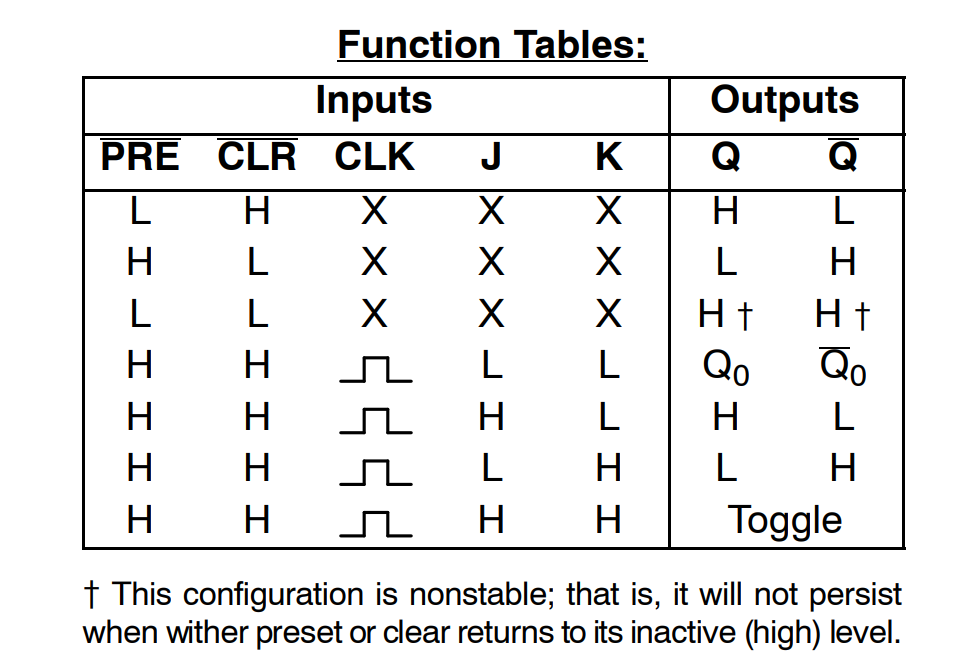
\includegraphics[scale = 0.5]{7476 function table.png}
	\caption{Function Table for IC 7476}
\end{figure}

\section{Pin Diagrams of ICs Used}

\subsection{Pin Diagram of IC7476}
\begin{figure}[H]
	\centering
	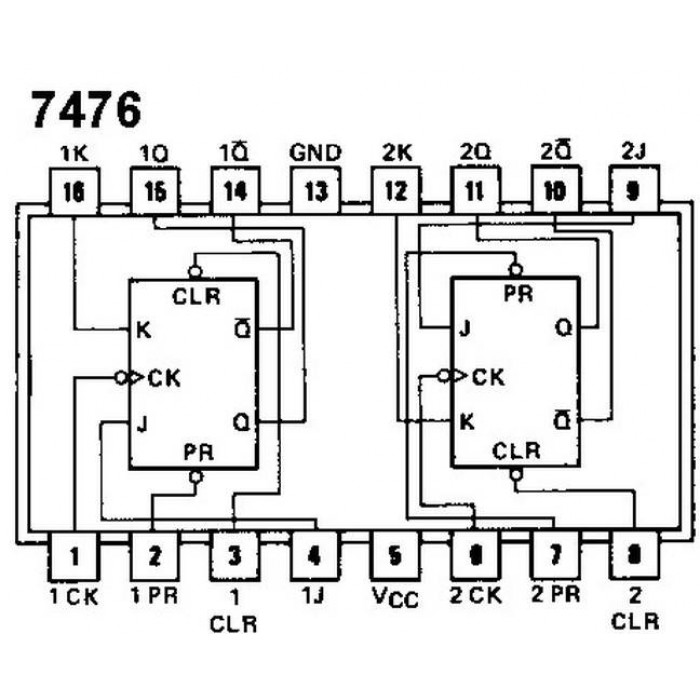
\includegraphics[scale = 0.35]{7476.jpg}
	\caption{Pin Diagram for IC 7476}
\end{figure}
\subsection{Pin Diagram of IC7400}
\begin{figure}[H]
	\centering
	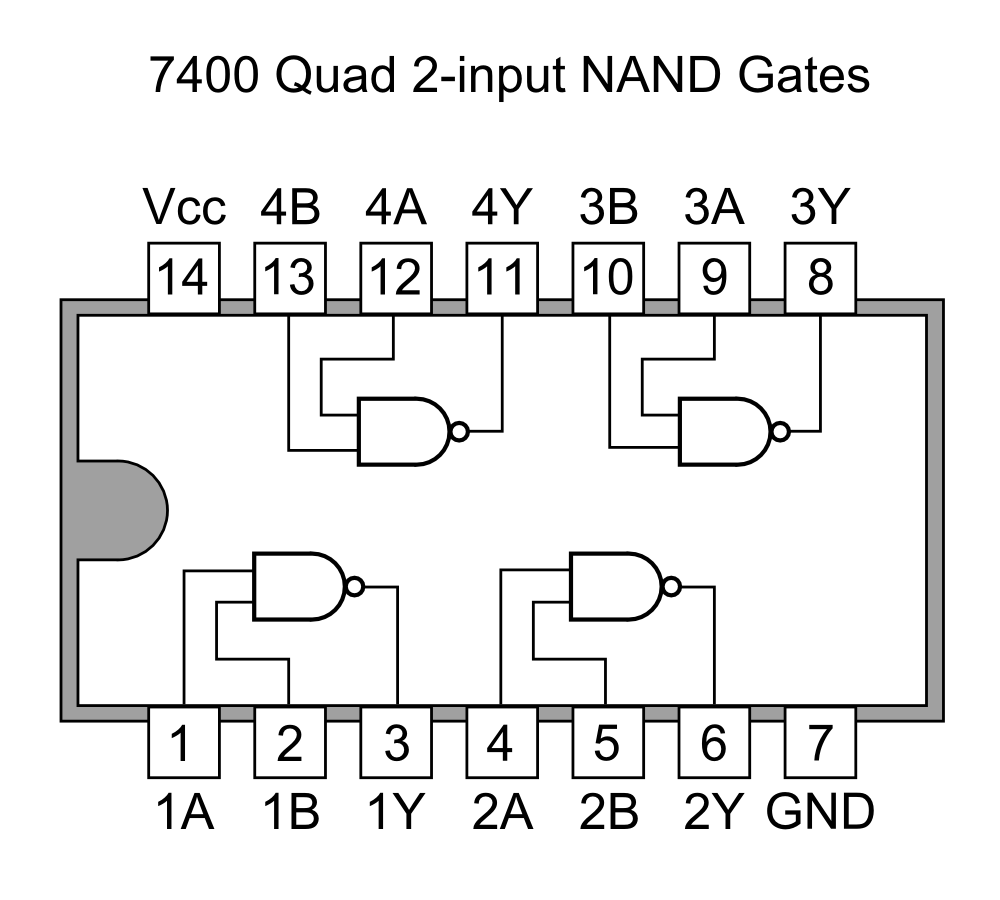
\includegraphics[scale = 0.25]{7400.png}
	\caption{Pin Diagram for IC 7400}
\end{figure}
\subsection{Timing diagram of a 3-bit asynchronous counter}
\begin{figure}[H]
	\centering
	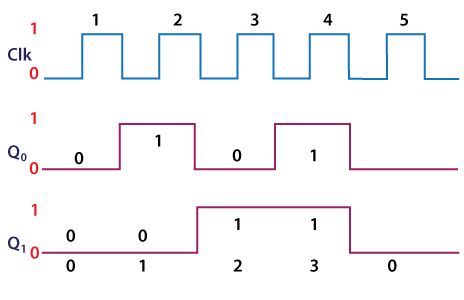
\includegraphics[scale = 0.55]{counters4.png}
	\caption{Timing diagram of a 3-bit asynchronous counter}
\end{figure}
\section{Design and Implementation}

\subsection{Circuit diagram of a 3-bit asynchronous counter: (3 Bit Asynchronous - UP Counter / Modulus 8)}
\begin{figure}[H]
	\centering
	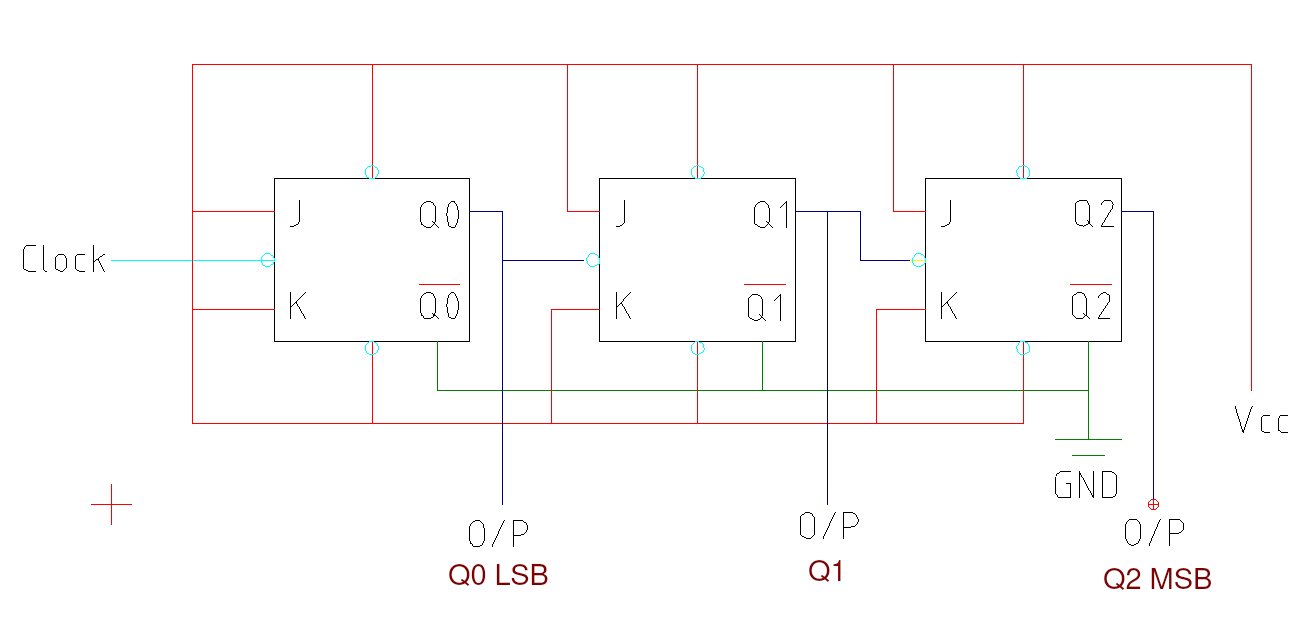
\includegraphics[scale = 0.5]{asynchronuos counter mod 8 up.png}
	\caption{Circuit diagram of a 3-bit asynchronous counter - UP}
\end{figure}

\subsection{Circuit diagram of a 3-bit asynchronous counter: (3 Bit Asynchronous - DOWN Counter / Modulus 8)}


\begin{figure}[H]
	\centering
	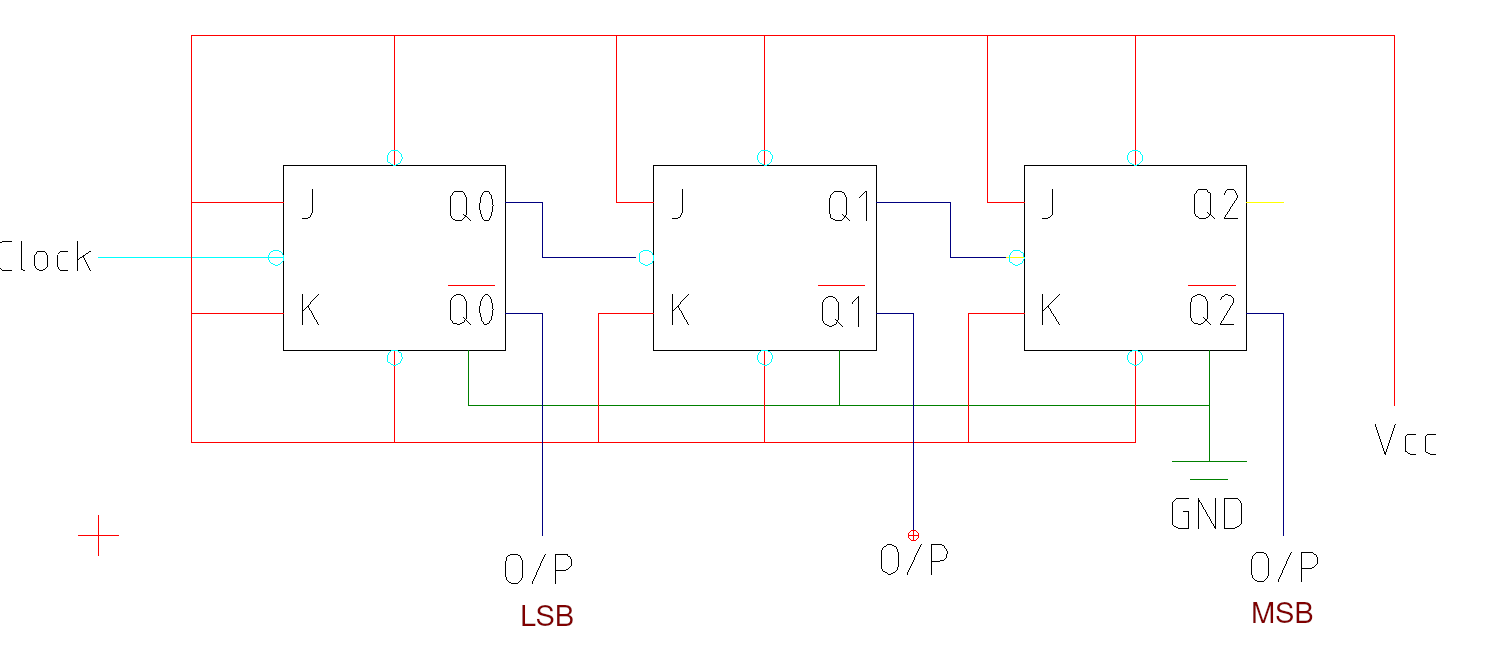
\includegraphics[scale = 0.45]{asynchronuos counter mod 8 down.png}
	\caption{Circuit diagram of a 3-bit asynchronous counter - Down}
\end{figure}
\subsection{Circuit Diagram MOD 5 (101) UP Asynchronous Counter - (Truncated Counter) using JK- Flip flop}

\begin{figure}[H]
	\centering
	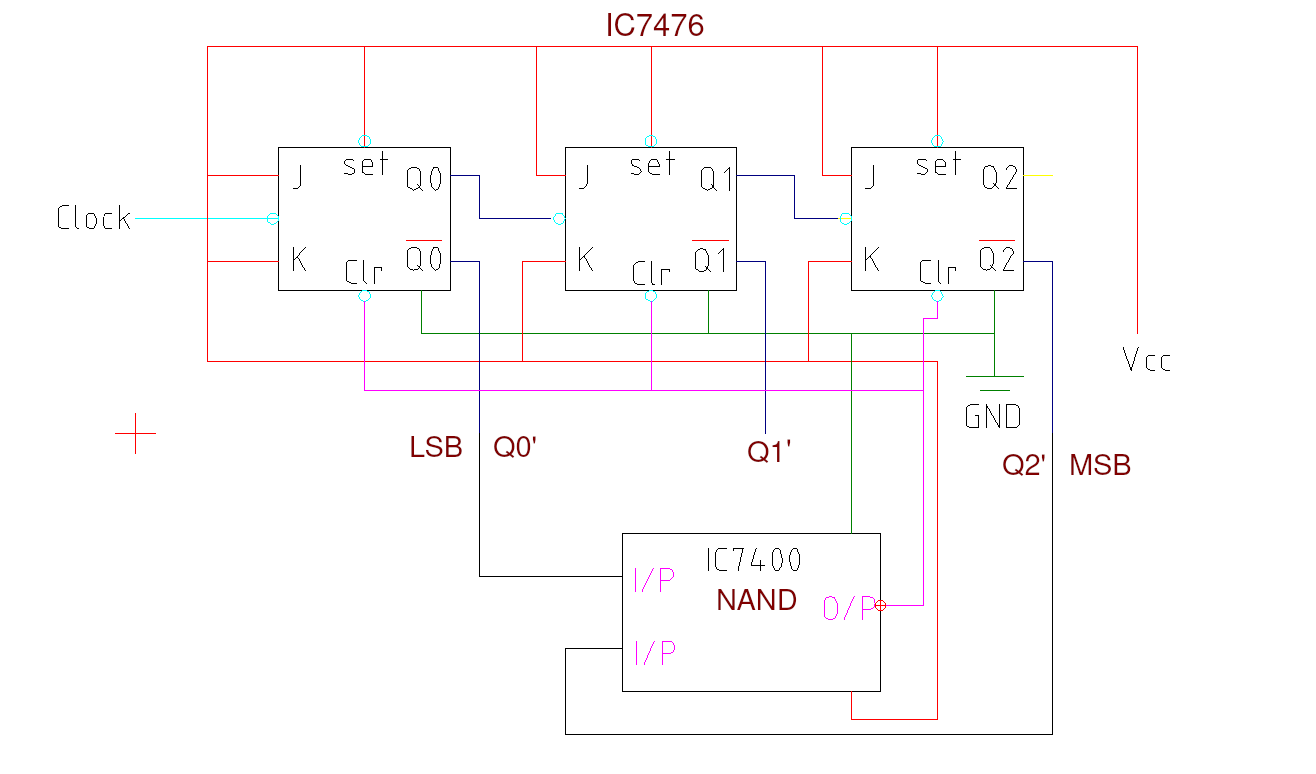
\includegraphics[scale = 0.5]{mod 5 counter.png}
	\caption{Circuit diagram of a 3-bit Mod Counter}
\end{figure}

\section{Procedure}

\begin{enumerate}
	\item Design Sequential circuit logic circuit as per given problem statement.
	\item Connect the IC 74LS76 and other basic logic gate ICs as per diagram.
	\item Give VCC supply and ground connection to each IC.
	\item Give clock to first JK FF.
	\item Observe the output and verify the truth table.
	\item Switch off the power supply of trainer kit.
\end{enumerate}

\section{Conclusion}
\textit{Thus, we have learnt a fundamental application and working of the IC 7476, and verified the truth table of its dual Master Slave JK Flip Flops. The Logic of Flip Flops was understood in detail, and implemented on the Digital Trainer Kit. Asynchronous counters were also implemented with MOD 8 and MOD 5 as 2 Separate Circuits on the Trainer kit. Their results were observed, noted and understood. }
\pagebreak

\section{FAQs}

\begin{enumerate}
	\item \textbf{One of the major drawbacks to the use of asynchronous counters is?}\\
	While counting large number of bits, the propagation delay of asynchronous counters is very large.	For high clock frequencies, counting errors may occur, due to propagation delay.	
	\item \textbf{How many flip-flops are required to construct a decade counter?}\\
	In Binary we can count to 10 in just 4 bits, and so 4 Bit Asynchronous counter is to be implemented. That means we would require 4 Flip Flops, 1 for each bit. 
	\item \textbf{The terminal count of a typical modulus 10 binary counter is?}\\
	The Terminal Count of a Typical Mod 10 Binary counter is 9, which would be represented as 1001
\end{enumerate}

\end{document}